\mode*

\section{Matriser}

\subsection{Lösa linjära ekvationssystem}

\begin{frame}
  \begin{equation*}
    \systeme*{
      x + 2y = 1,
      3x + 4y = 2
    }
    \qquad\equiv\qquad
    \systeme*{
      x_0 + 2x_1 = 1,
      3x_0 + 4x_1 = 2
    }
  \end{equation*}
\end{frame}

\begin{frame}
  \begin{equation*}
    \systeme*{
      x_0 + 2x_1 = 1,
      3x_0 + 4x_1 = 2
    }
    \quad\equiv\quad
    \begin{bmatrix}
      1 & 2 \\
      3 & 4
    \end{bmatrix}
    \begin{bmatrix}
      x_0 \\
      x_1
    \end{bmatrix}
    =
    \begin{bmatrix}
      1 \\
      2
    \end{bmatrix}
    \quad\equiv\quad
    \vect{A}\vect{x} = \vect{b}
  \end{equation*}
\end{frame}

\begin{frame}[fragile]
  \inputminted[linenos,lastline=4]{python}{examples/solve.py}
  \dots
  \inputminted[linenos,firstline=15,lastline=22]{python}{examples/solve.py}
\end{frame}

\begin{frame}[fragile]
  \inputminted[linenos,firstline=6,lastline=14]{python}{examples/solve.py}
\end{frame}


\subsection{Hitta rötter}

\begin{frame}
  \begin{block}{Problem}
    \begin{itemize}
      \item Låt \(f(x) = (x-1)(x+2) = x^2 + x -2\).
      \item Hitta \(x\) sådant att \(f(x) = 0\).
    \end{itemize}
  \end{block}
\end{frame}

\begin{frame}[fragile]
  \inputminted[linenos,firstline=1,lastline=3]{python}{examples/nr.py}
  \dots
  \inputminted[linenos,firstline=18,lastline=23]{python}{examples/nr.py}
\end{frame}

\begin{frame}
  \begin{definition}[Newton-Raphsons metod]
    \begin{itemize}
      \item Vill hitta \(f(x) = 0\).
      \item Gissa \(x_0\).
      \item Låt \(x_{n+1} = x_n - \frac{f(x_n)}{f'(x_n)}\)
      \item När \(|x_{n+1} - x_n|\) är \enquote{litet} kommer \(f(x_{n+1})\) 
        att vara nära noll.
    \end{itemize}
  \end{definition}
\end{frame}

\begin{frame}[fragile]
  \inputminted[linenos,firstline=5,lastline=15]{python}{examples/nr.py}
\end{frame}


\section{Grafer}

\begin{frame}
  \begin{figure}
    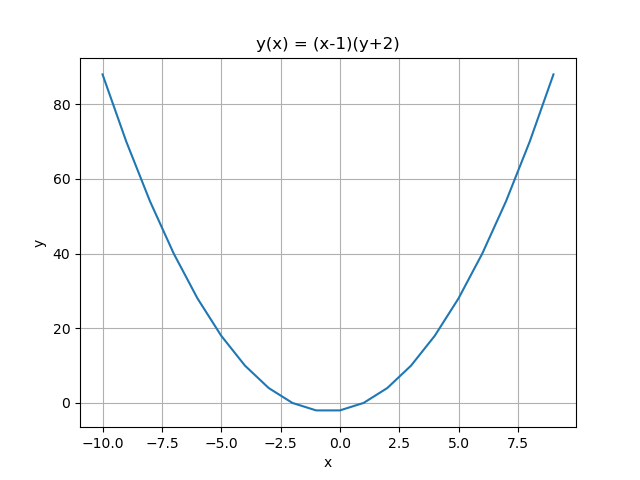
\includegraphics[height=0.8\textheight]{fig/plot_f.png}
    \caption{En graf för \(y(x) = (x-1)(x+2)\).}
  \end{figure}
\end{frame}

\begin{frame}
  \inputminted[linenos,lastline=16]{python}{examples/plot_f.py}
\end{frame}

\begin{frame}
  \begin{figure}
    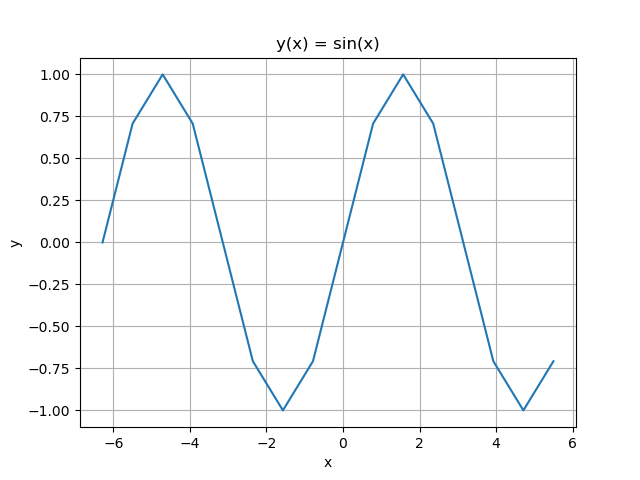
\includegraphics[height=0.8\textheight]{fig/plot_sin.png}
    \caption{En graf över \(y(x) = \sin(x)\).}
  \end{figure}
\end{frame}

\begin{frame}
  \inputminted[linenos,firstline=3,lastline=20]{python}{examples/plot_sin.py}
\end{frame}
